\documentclass[11pt]{article}
\usepackage{amsmath}
\usepackage{amssymb}
\usepackage{amsfonts}
\usepackage{geometry}
\geometry{margin=1in}
\usepackage{graphicx}

\title{Computational Neuroscience Homwork 3}
\author{Sepehr SAEEDPOUR}
\date{June 2025}

\begin{document}

\maketitle

\section{Hopfield Networks}

\subsection*{(a) the pattern $\xi$ is a fixed point}

\textbf{Assuming:}
\begin{itemize}
    \item Weight matrix: $w_{ij} = \frac{1}{N}(\xi_i\xi_j + \eta_i\eta_j)$
    \item Update rule: $y_i = \text{sgn}\left(\sum_{j=1}^N w_{ij} y_j\right)$
    \item Orthogonality condition: $\sum_{j=1}^N \xi_j \eta_j = 0$
\end{itemize}

% \textbf{Proof:}
To show $\xi$ is a fixed point, we need to demonstrate that when $y = \xi$, the update rule returns $y_i = \xi_i$ for all $i$.

Starting with the update rule when $y = \xi$:
\begin{equation}
y_i = \text{sgn}\left(\sum_{j=1}^N w_{ij} \xi_j\right)
\end{equation}

Substituting the weight matrix:
\begin{equation}
y_i = \text{sgn}\left(\sum_{j=1}^N \frac{1}{N}(\xi_i\xi_j + \eta_i\eta_j) \xi_j\right)
\end{equation}

\begin{equation}
= \text{sgn}\left(\frac{1}{N}\sum_{j=1}^N (\xi_i\xi_j^2 + \eta_i\eta_j\xi_j)\right)
\end{equation}

Since $\xi_j \in \{-1, +1\}$, we have $\xi_j^2 = 1$:
\begin{equation}
= \text{sgn}\left(\frac{1}{N}\left(\xi_i\sum_{j=1}^N 1 + \eta_i\sum_{j=1}^N\eta_j\xi_j\right)\right)
\end{equation}

\begin{equation}
= \text{sgn}\left(\frac{1}{N}\left(\xi_i \cdot N + \eta_i \cdot 0\right)\right)
\end{equation}

The second term equals zero due to the orthogonality condition $\sum_{j=1}^N \xi_j \eta_j = 0$.

Therefore:
\begin{equation}
y_i = \text{sgn}(\xi_i) = \xi_i
\end{equation}

This proves that $\xi$ is indeed a fixed point.

\subsection*{(b) the pattern $\eta$ is also a fixed point}

Following the same approach, when $y = \eta$:
\begin{equation}
y_i = \text{sgn}\left(\sum_{j=1}^N w_{ij} \eta_j\right)
\end{equation}

Substituting the weight matrix:
\begin{equation}
y_i = \text{sgn}\left(\sum_{j=1}^N \frac{1}{N}(\xi_i\xi_j + \eta_i\eta_j) \eta_j\right)
\end{equation}

\begin{equation}
= \text{sgn}\left(\frac{1}{N}\sum_{j=1}^N (\xi_i\xi_j\eta_j + \eta_i\eta_j^2)\right)
\end{equation}

Since $\eta_j^2 = 1$:
\begin{equation}
= \text{sgn}\left(\frac{1}{N}\left(\xi_i\sum_{j=1}^N\xi_j\eta_j + \eta_i\sum_{j=1}^N 1\right)\right)
\end{equation}

\begin{equation}
= \text{sgn}\left(\frac{1}{N}\left(\xi_i \cdot 0 + \eta_i \cdot N\right)\right)
\end{equation}

Again, the first term equals zero due to orthogonality.

Therefore:
\begin{equation}
y_i = \text{sgn}(\eta_i) = \eta_i
\end{equation}

This proves that $\eta$ is also a fixed point.

\subsection*{(c) Intuitive explanation of why orthogonality reduces interference}

The orthogonality condition $\sum_{j=1}^N \xi_j \eta_j = 0$ ensures that the two stored patterns are maximally different from each other. When the network tries to retrieve one pattern, the contribution from the other pattern in the weight matrix cancels out exactly.

When the stored patterns are not orthogonal, trying to recall pattern $\xi$ also picks up stray influence from pattern $\eta$, nudging some neurons toward the wrong value. This extra “crosstalk” can create mixed, spurious states, shrink the safe region from which each memory can be recovered, and generally make recall less reliable—especially if you begin with a noisy or incomplete cue.

The orthogonality condition maximizes the separation between patterns in the neural state space, making each pattern's basin of attraction as large and well-defined as possible.

\section{Rate-based Dynamics Equivalence}

\textbf{We have:}
\begin{align}
\dot{r} &= -r + \phi(Jr) \\
\dot{v} &= -v + J\phi(v) \\
\end{align}

Starting with the first equation and applying the change of variables $v = Jr$:

Since $v = Jr$, we have $r = J^{-1}v$ (assuming $J$ is invertible).

Taking the time derivative: $\dot{v} = J\dot{r}$

Substituting into the first equation:
\begin{equation}
\dot{r} = -r + \phi(Jr) = -J^{-1}v + \phi(v)
\end{equation}

Multiplying both sides by $J$:
\begin{equation}
J\dot{r} = -v + J\phi(v)
\end{equation}

Since $\dot{v} = J\dot{r}$:
\begin{equation}
\dot{v} = -v + J\phi(v)
\end{equation}

This is exactly the second equation, proving mathematical equivalence.

In the first formulation, $r$ represents firing rates, and $Jr$ represents the total synaptic input. In the second formulation, $v$ represents membrane potentials directly. The transformation $v = Jr$ links these two perspectives: membrane potential equals the weighted sum of presynaptic firing rates


\section{Leak in Linear Dynamical Systems}

\subsection*{(a) Effect of leak term on eigenvalues}

\textbf{The system is:} $\dot{x}(t) = -x(t) + Jx(t) = (J - I)x(t)$

So $A = J - I$.

If $Jv = \lambda_i v$ for some eigenvector $v$, then:
\begin{equation}
Av = (J - I)v = Jv - Iv = \lambda_i v - v = (\lambda_i - 1)v
\end{equation}

Therefore, $A$ has the same eigenvectors as $J$, but each eigenvalue is shifted by $-1$. 
If $J$ has eigenvalues $\lambda_i$, then $A$ has eigenvalues $\lambda_i - 1$.




The leak term $-x(t)$ shifts all eigenvalues to the left in the complex plane by 1 unit. 
This makes the system more stable (eigenvalues become more negative), introduces a restoring force that pulls activity toward zero, and prevents unbounded growth even if $J$ has eigenvalues $> 0$.


\subsection*{(b) Stability condition and effect of removing leak}

For the full system $\dot{x}(t) = (J - I)x(t)$ to be stable, all eigenvalues of $A = J - I$ must have negative real parts.

Since the eigenvalues of $A$ are $\lambda_i - 1$ where $\lambda_i$ are the eigenvalues of $J$, the stability condition is:
\begin{equation}
\text{Re}(\lambda_i - 1) < 0 \quad \text{for all } i
\end{equation}

This simplifies to:
\begin{equation}
\text{Re}(\lambda_i) < 1 \quad \text{for all } i
\end{equation}


When the leak is removed, the system becomes $\dot{x} = Jx$.

In this case, the system is stable only if $\text{Re}(\lambda_i) < 0$ for all eigenvalues of $J$ and any eigenvalue with $\text{Re}(\lambda_i) \geq 0$ will cause exponential growth. 
    Without the leak term, small perturbations can lead to unbounded dynamics.

The leak term essentially provides a ``safety margin'' of 1 unit in the real part of eigenvalues, allowing the system to remain stable even when $J$ has eigenvalues with positive real parts (as long as $\text{Re}(\lambda_i) < 1$).




\textbf{Numerical verification:}

Figure~\ref{fig:eigenvalue_analysis} illustrates the stability characteristics of a system by plotting the eigenvalues of matrices $J$ and $A = J - I$ in the complex plane. In the left panel, the eigenvalues of $J$ are shown with a vertical dashed line at $\text{Re} = 1$, marking the stability boundary for a system that includes a leak term. The right panel displays the eigenvalues of $A$, which are shifted left by one unit compared to those of $J$, with the stability boundary now at $\text{Re} = 0$. This shift aligns with theoretical expectations, as subtracting the identity matrix from $J$ reduces the real part of each eigenvalue by one.

\begin{figure}[h]
\centering
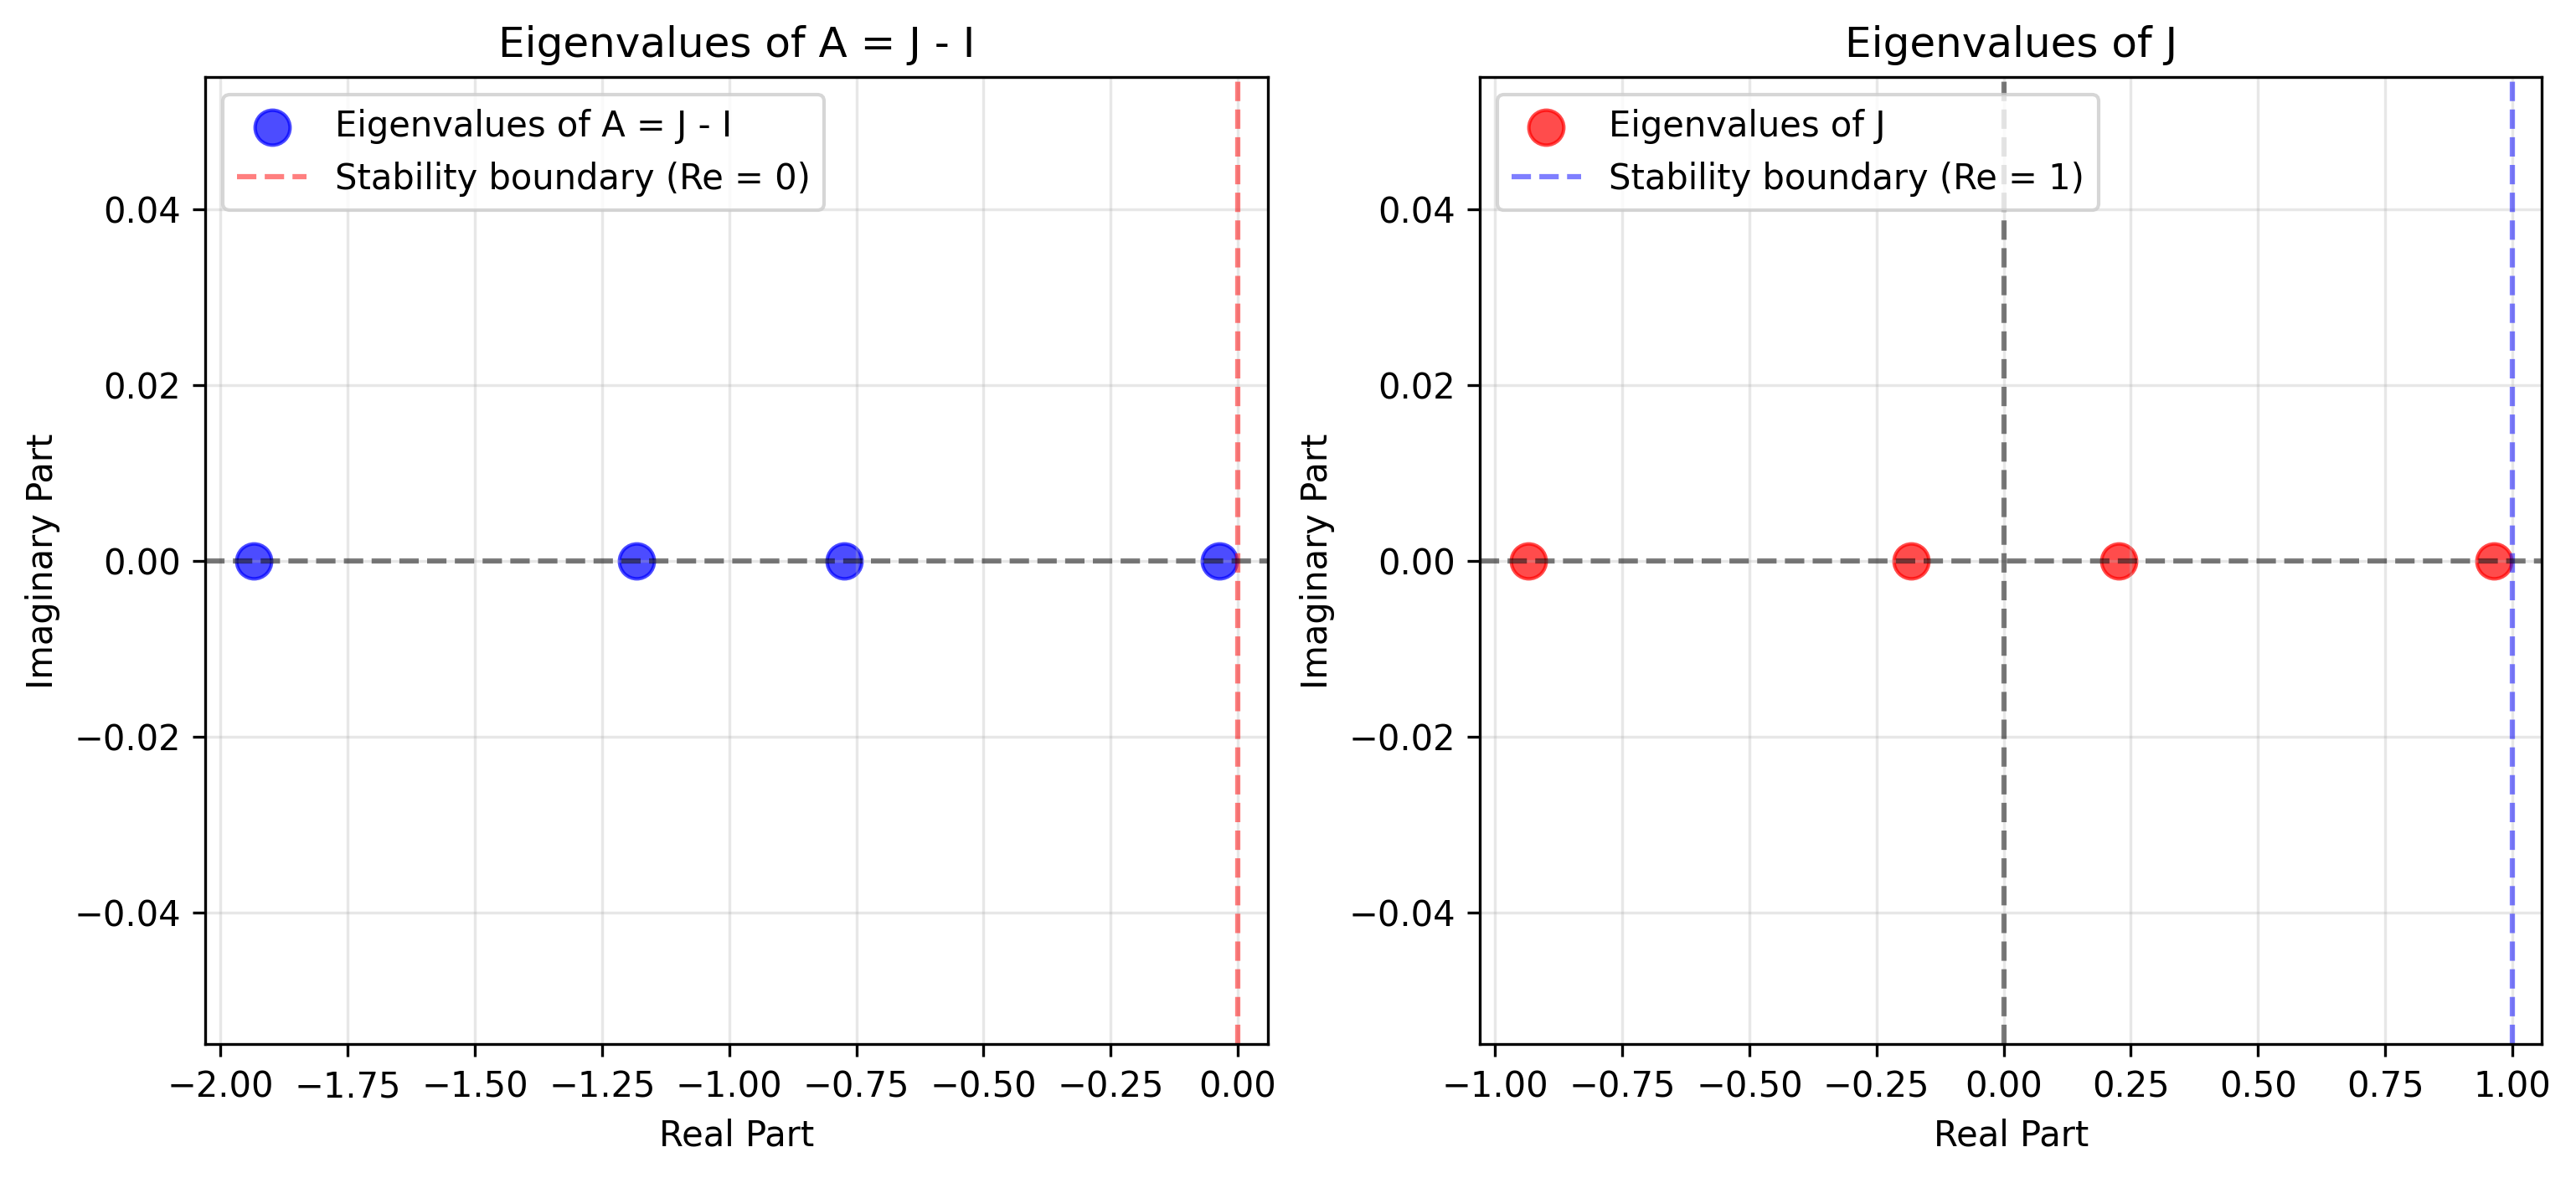
\includegraphics[width=0.6\textwidth]{eigenvalues_comparison.png}
\caption{Eigenvalue analysis demonstrating the effect of leak on system stability. Right: Eigenvalues of matrix $J$ with stability boundary at $\text{Re} = 1$. Left: Eigenvalues of $A = J - I$ with stability boundary at $\text{Re} = 0$. The leak term shifts all eigenvalues left by 1 unit, providing a stability margin.}
\label{fig:eigenvalue_analysis}
\end{figure}


Figure~\ref{fig:dynamics_comparison} shows the temporal evolution of the system norm $\|x(t)\|$ for multiple initial conditions, comparing dynamics with and without the leak term. The left panel demonstrates that the system with leak ($\dot{x} = (J-I)x$) exhibits stable behavior with trajectories converging to zero, while the right panel shows that the system without leak ($\dot{x} = Jx$) can exhibit exponential growth when eigenvalues of $J$ have positive real parts.

\begin{figure}[h]
\centering
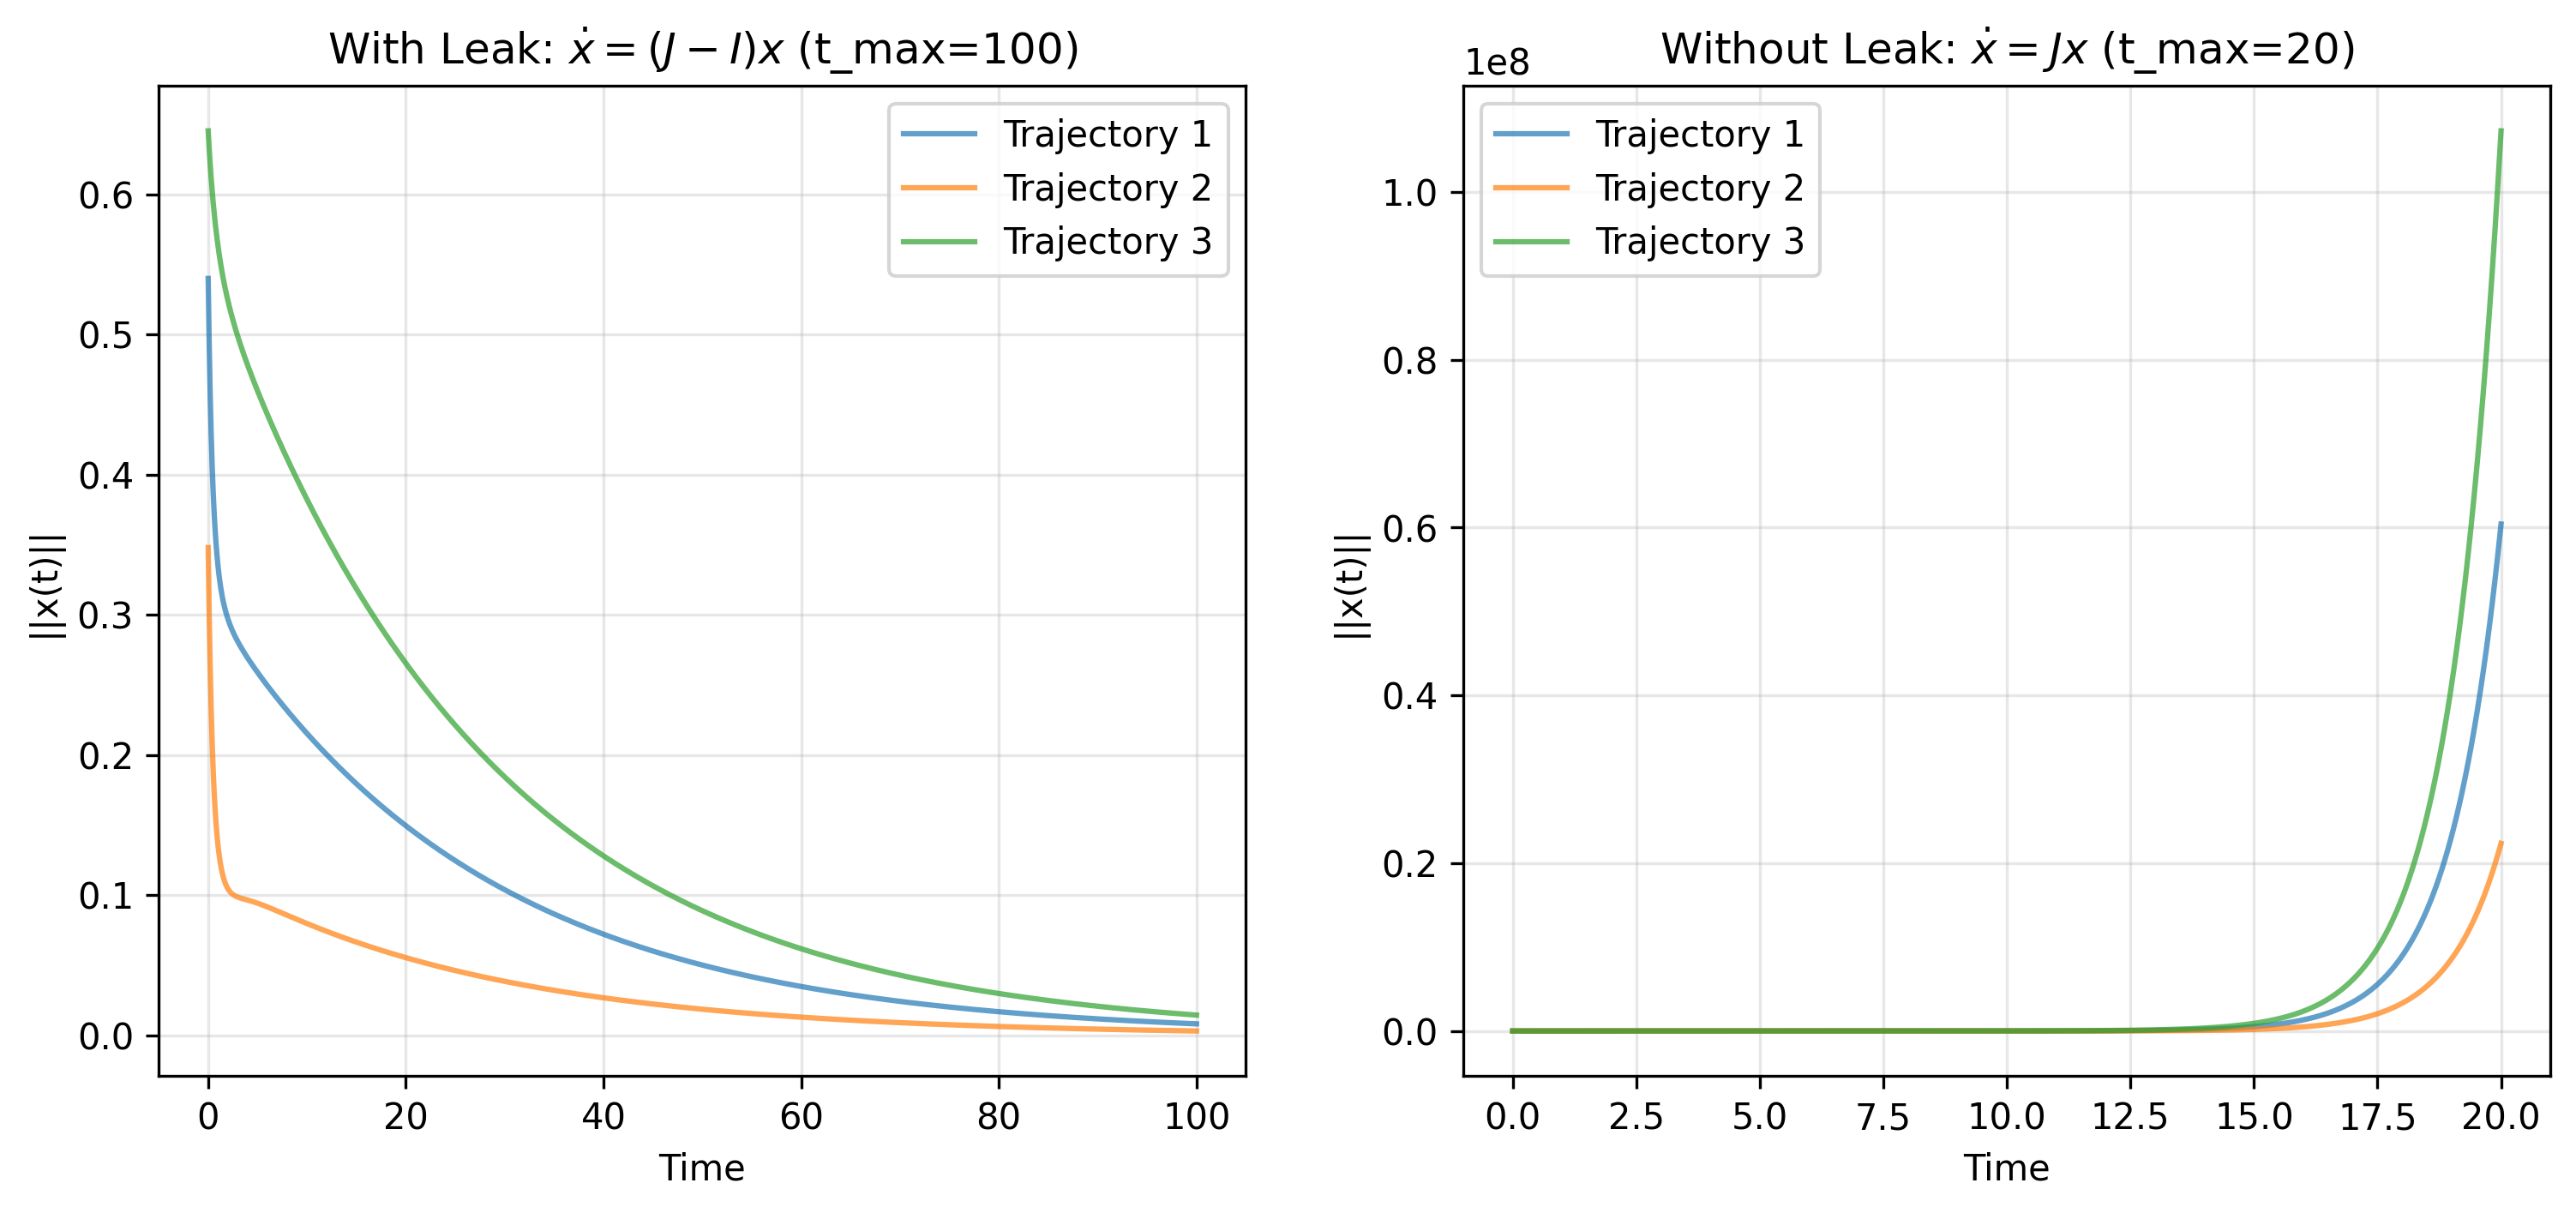
\includegraphics[width=0.6\textwidth]{dynamics_comparison.png}
\caption{Comparison of system dynamics with and without leak term. Left: System with leak shows stable convergence to zero for all trajectories. Right: System without leak exhibits exponential growth due to eigenvalues with positive real parts. The leak term provides crucial stabilization of the dynamics.}
\label{fig:dynamics_comparison}
\end{figure}


\subsection*{Nonlinear RNN for cognitive tasks}

\subsubsection*{(c)}

For training the network, I used PerceptualDecisionMaking-v0 task.
Basically, PerceptualDecisionMaking-v0 simulates the classic random-dot-motion two-alternative forced-choice paradigm in silico, presenting the network with a cloud in which a tunable fraction of dots drifts coherently left or right while the remainder jitters randomly, so embedding a weak directional signal in noise. 
The stimulus is encoded as two continuously fluctuating input channels whose moment-by-moment means differ by the signed “coherence,” so the only route to high accuracy is to accumulate this differential evidence until an internal decision variable hits a bound, precisely the computation formalised by the drift-diffusion model and replicated in attractor-network simulations of perceptual choice.

Training success was assessed by monitoring the loss function and accuracy over epochs. 
A successful training run showed a decreasing loss and increasing accuracy, plateauing near 99\% accuracy on training sets (see Figure~\ref{fig:training_performance}) .
Training success was also assessed using a psychometric function, which plots choice accuracy as a function of stimulus coherence, showing how the network's decision-making ability scales with signal strength (see Figure~\ref{fig:psychometric_function}).


\begin{figure}[h]
\centering
\begin{minipage}{0.48\textwidth}
    \centering
    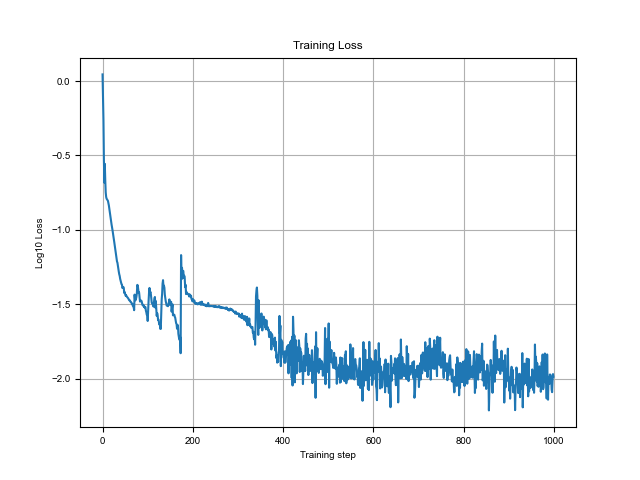
\includegraphics[width=\textwidth]{training_loss.png}
\end{minipage}
\hfill
\begin{minipage}{0.48\textwidth}
    \centering
    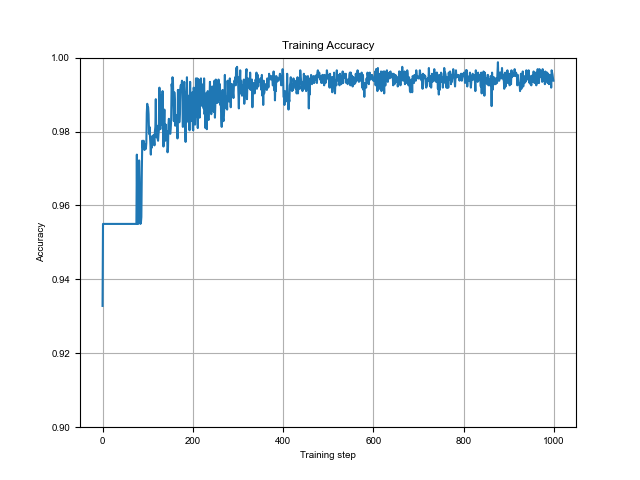
\includegraphics[width=\textwidth]{training_accuracy.png}
\end{minipage}
\caption{Training performance of the nonlinear RNN on the perceptual decision-making task. Left: Cross-entropy loss decreases over training epochs, showing effective optimization. Right: Task accuracy increases from chance level to nearly 99\%, indicating successful learning of the evidence accumulation process required for distinguishing motion direction in noisy visual stimuli.}
\label{fig:training_performance}
\end{figure}


\begin{figure}[h]
\centering
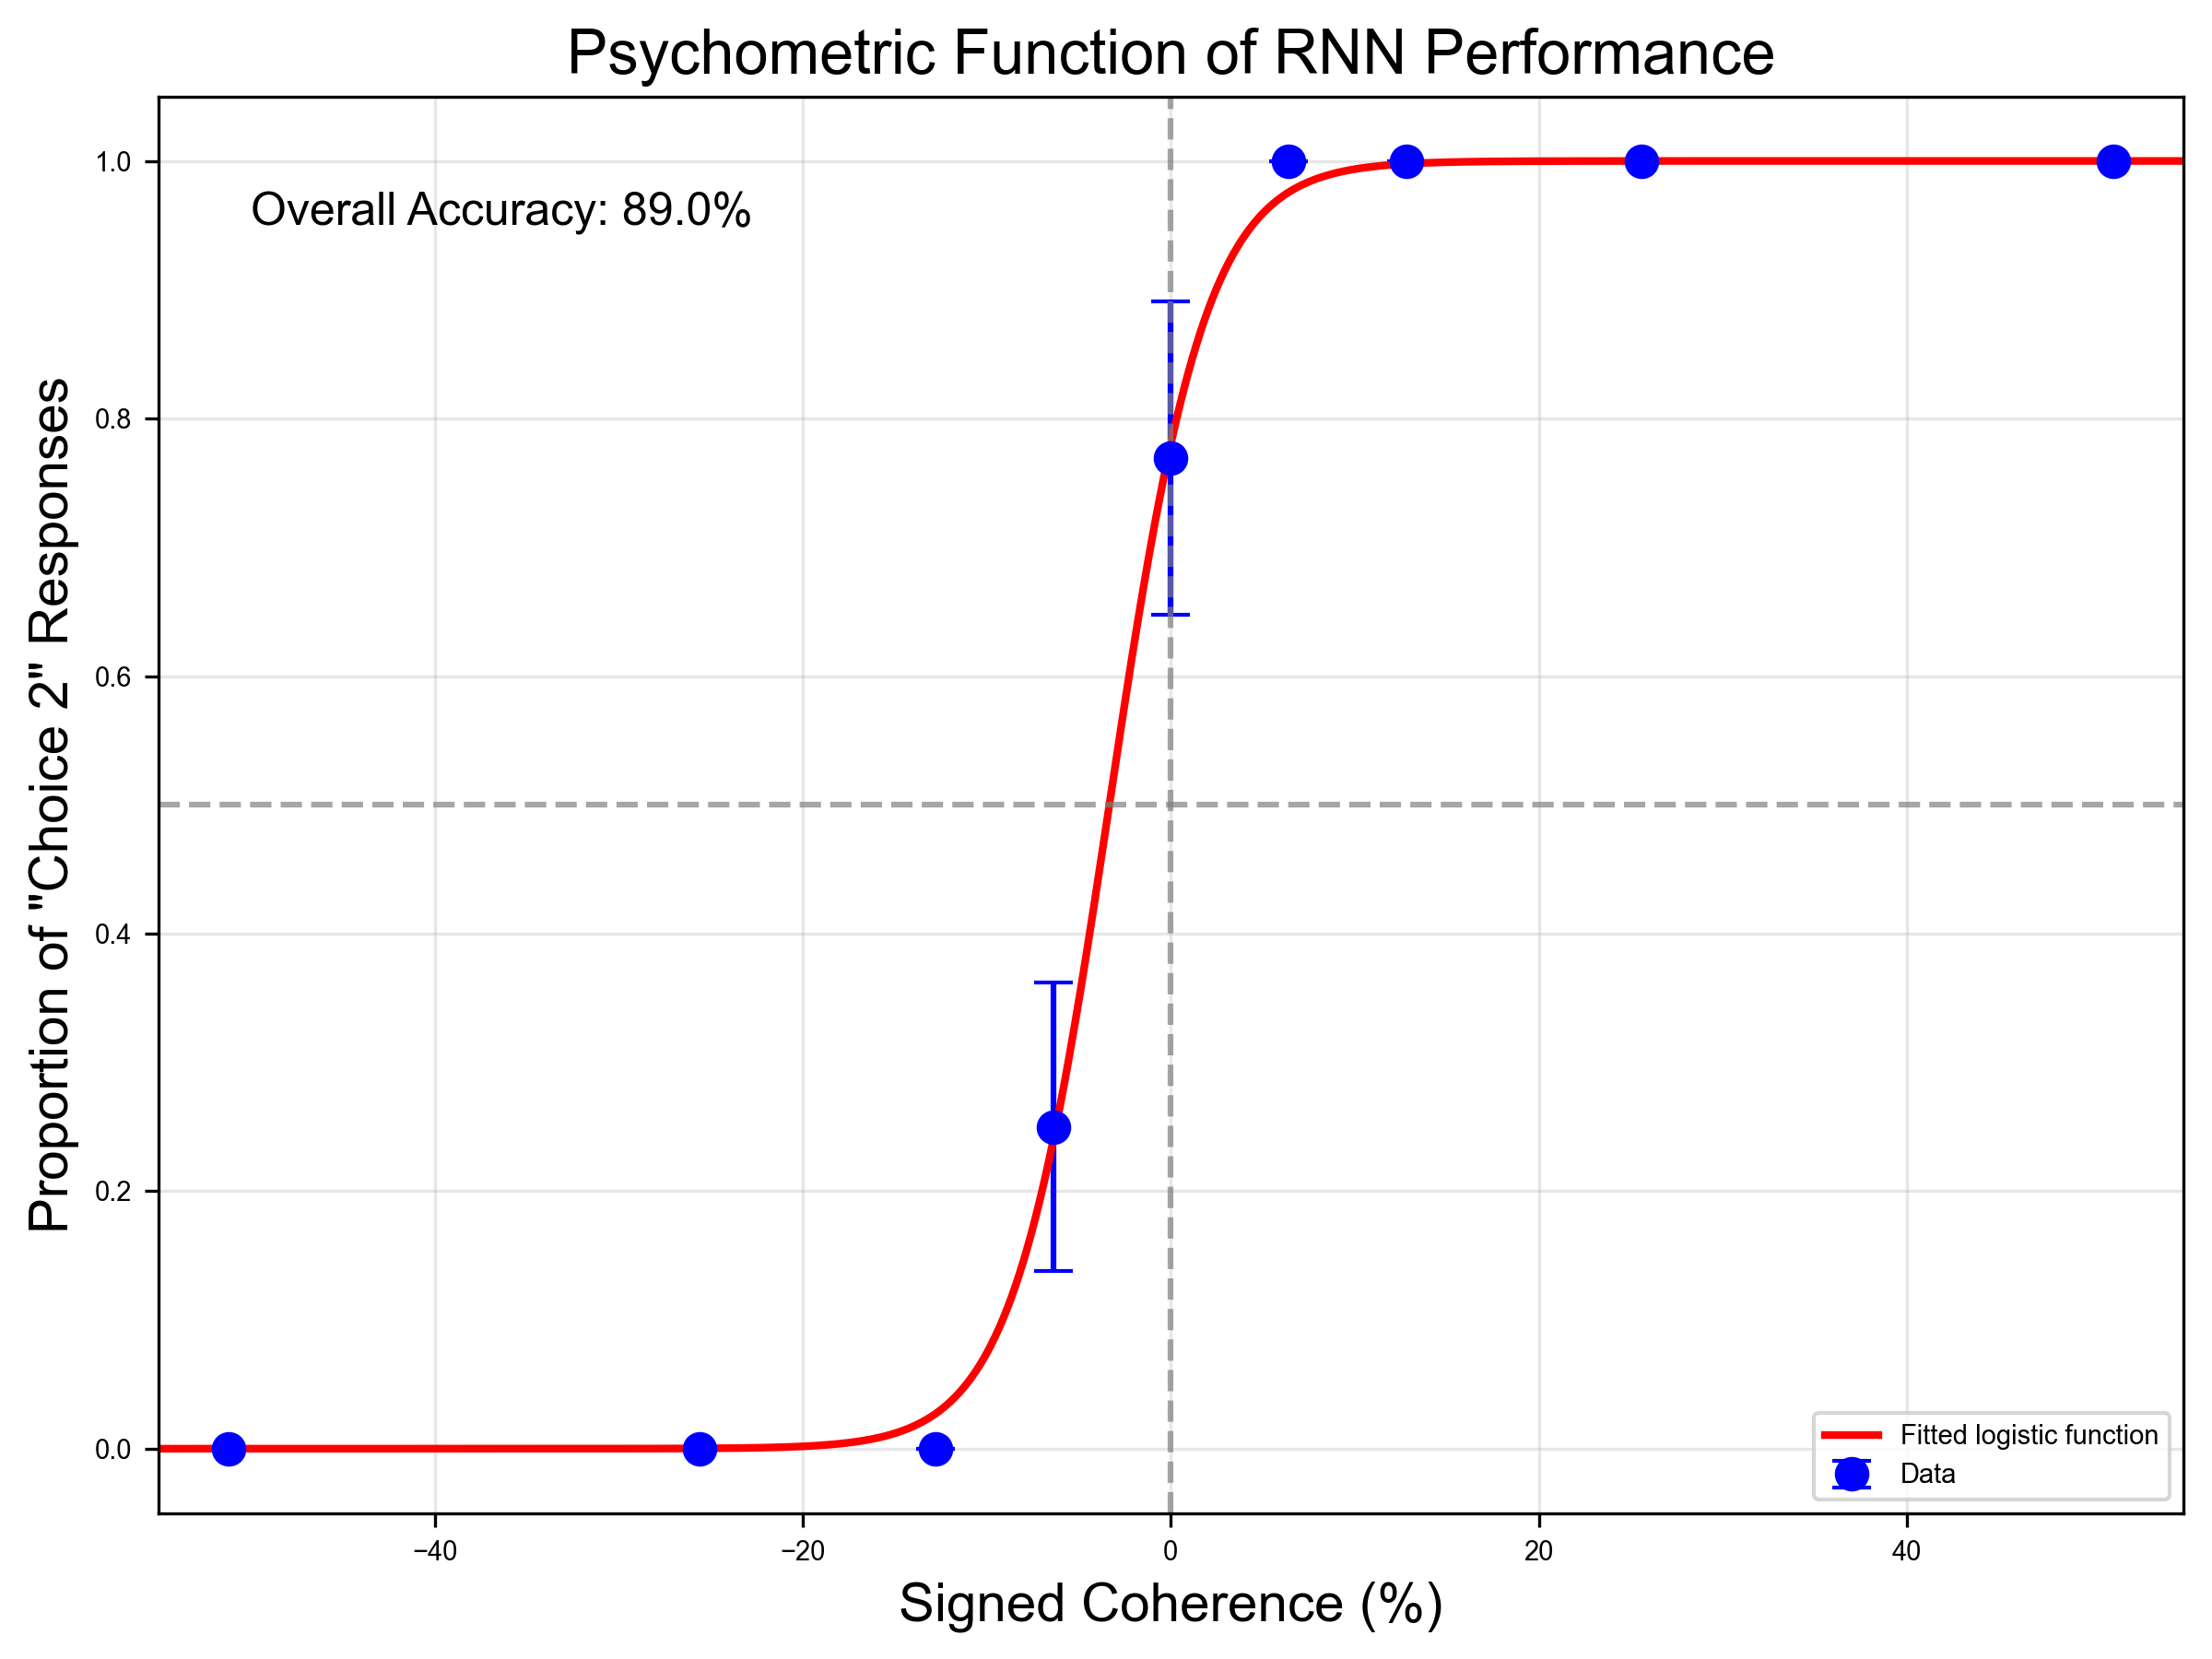
\includegraphics[width=0.6\textwidth]{psychometric_function.png}
\caption{Psychometric function of the trained RNN model on the perceptual decision-making task. The x-axis represents stimulus coherence (strength of motion signal), while the y-axis shows choice accuracy. The network exhibits the characteristic sigmoidal relationship between signal strength and performance, with chance-level performance (50\%) at zero coherence and near-perfect accuracy at high coherence levels, demonstrating successful learning of evidence accumulation. This characteristic S-shaped curve closely resembles the psychometric functions observed in both human and animal subjects performing perceptual decision-making tasks.}
\label{fig:psychometric_function}
\end{figure}

\pagebreak


\subsubsection*{(d)}

After training, I analyzed the RNN's internal dynamics using Principal Component Analysis (PCA) to reduce the dimensionality of the hidden state activity. This revealed distinct trajectories in the principal component space corresponding to different trial types (e.g., left vs. right choices). Such separation suggests that the RNN encodes different stimuli in separable subspaces, facilitating accurate decision-making.

Figure~\ref{fig:pca_trajectories} illustrates the trajectories of the RNN hidden states projected onto the first three principal components during different trials. The clear separation between left-choice and right-choice trajectories demonstrates that the network forms distinct neural representations for different decision outcomes to solve the task. 

\begin{figure}[h]
\centering
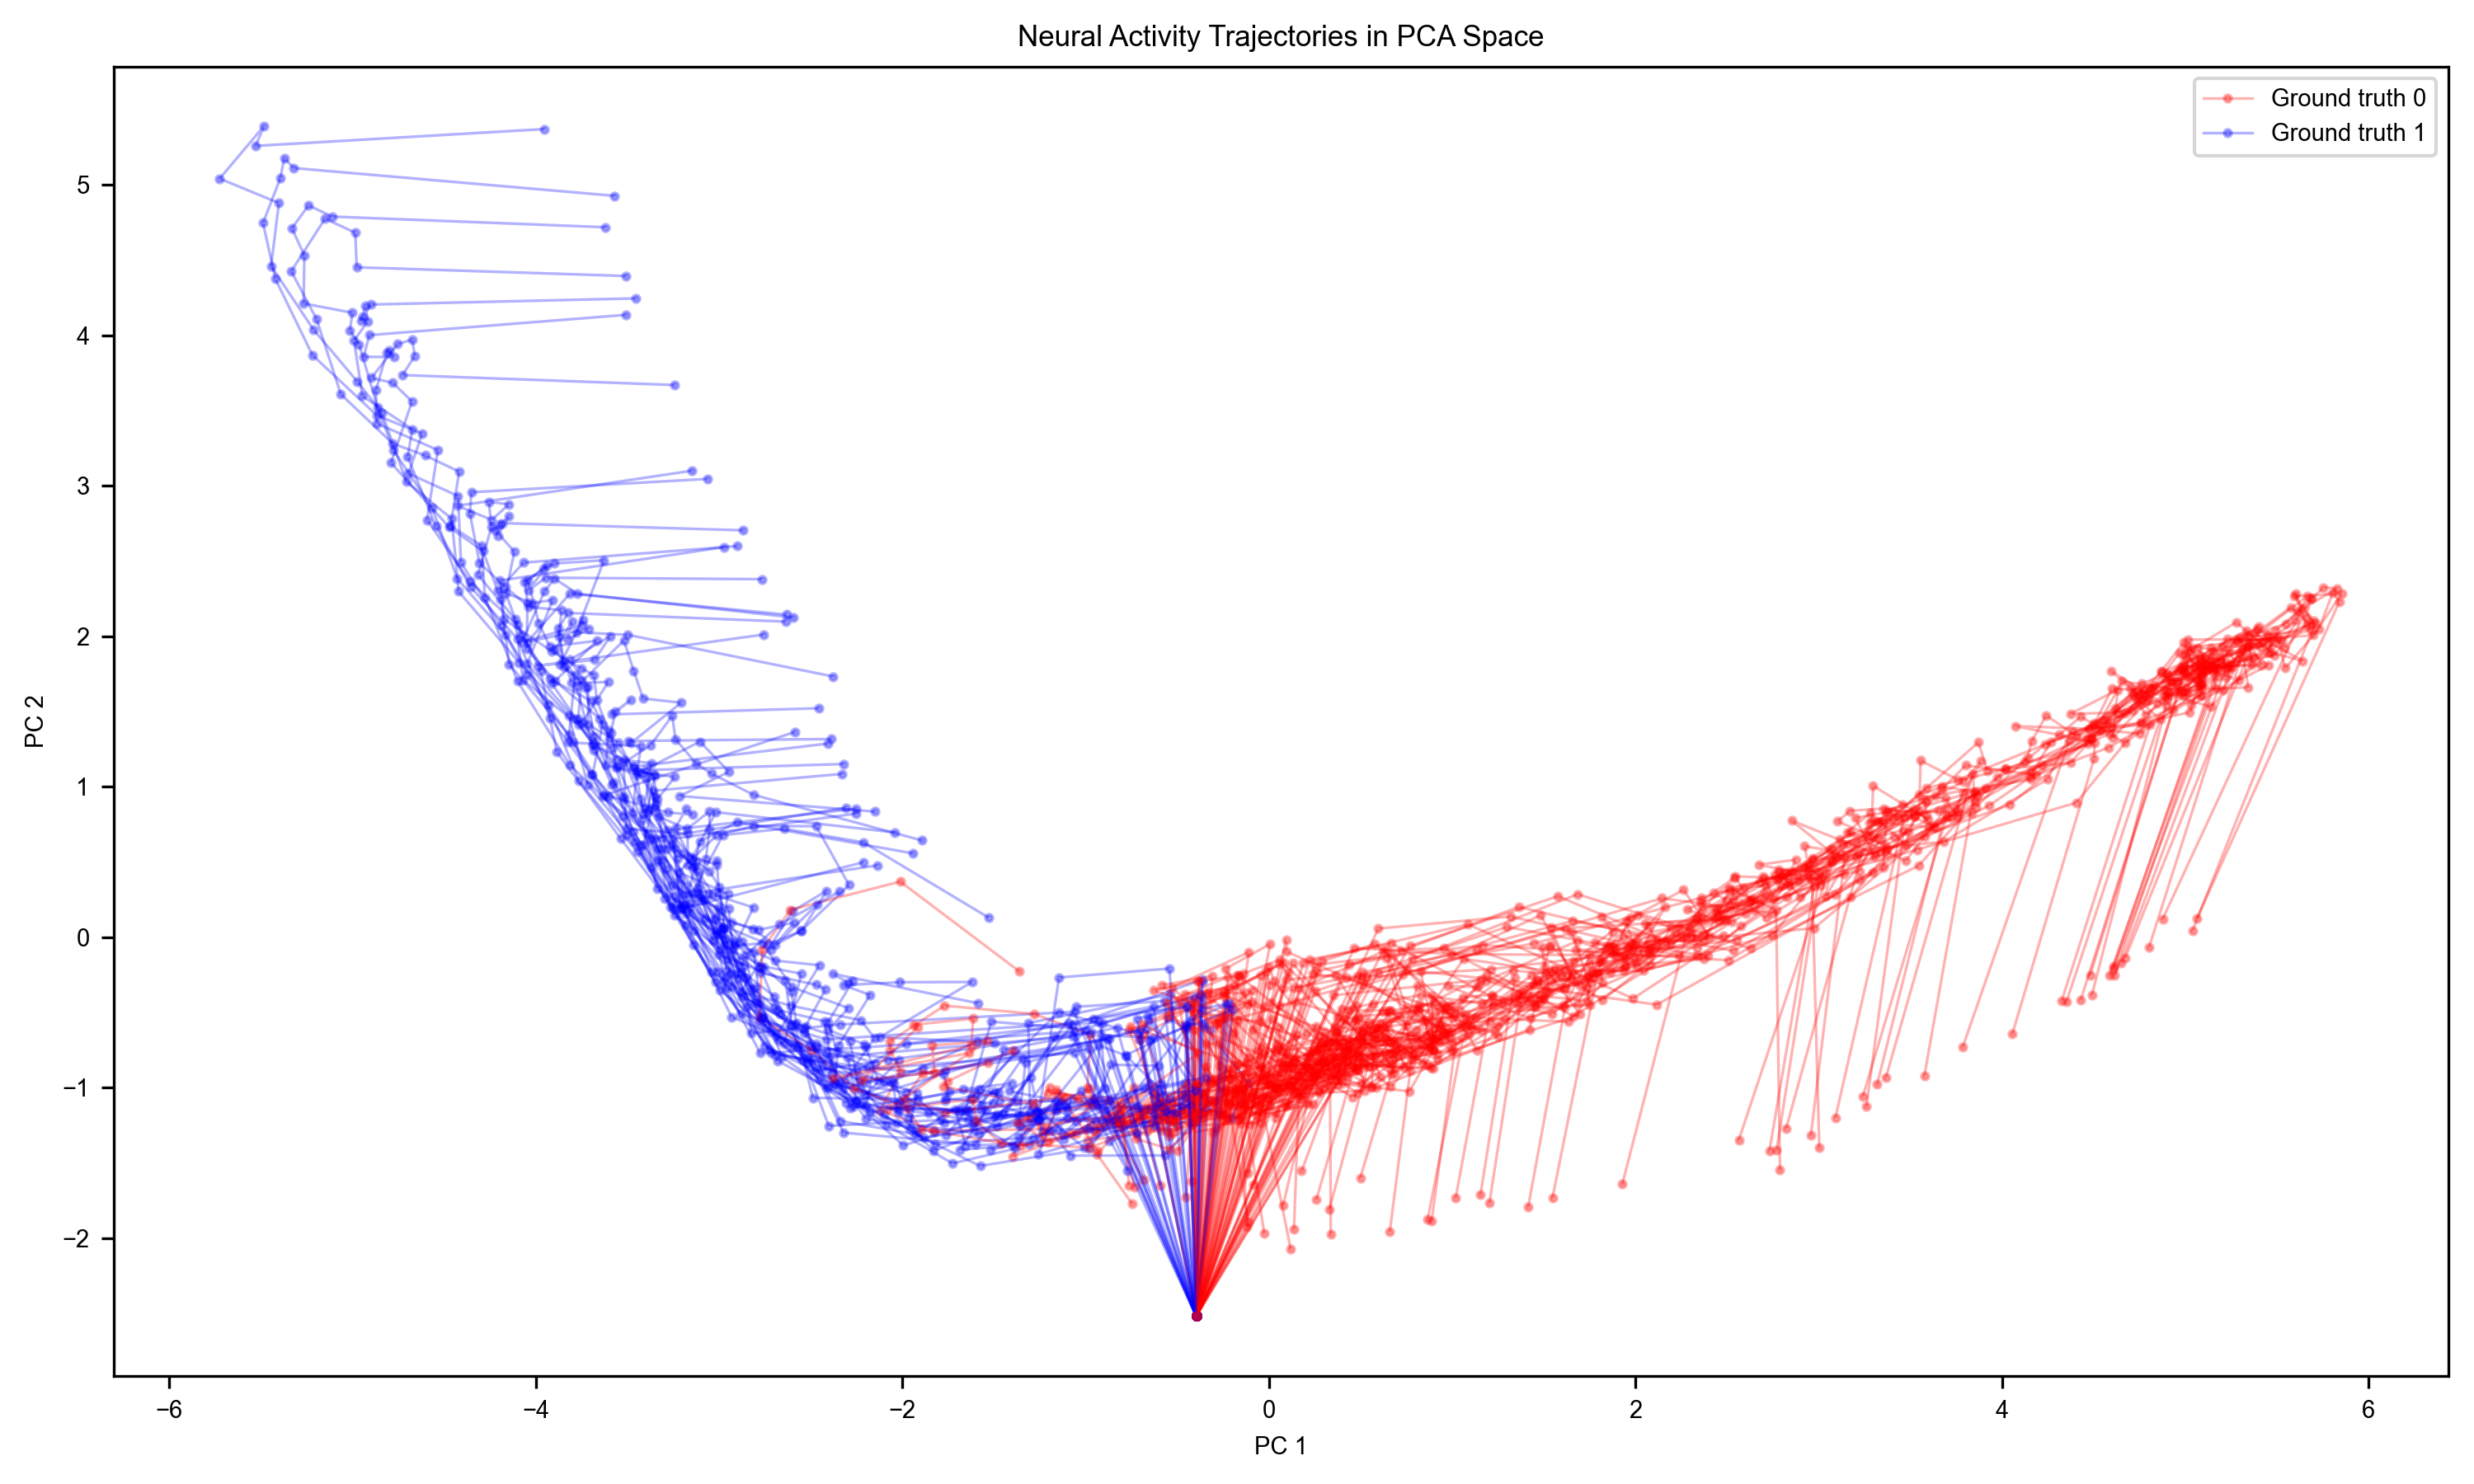
\includegraphics[width=0.7\textwidth]{pca_trajectory.png}
\caption{PCA trajectories of RNN hidden states during perceptual decision-making. Different colors represent different trial types (blue: rightward motion stimuli, red: leftward motion stimuli). The trajectories start close together early in the trial and gradually separate as evidence accumulates, eventually settling into distinct regions of the state space corresponding to the two possible decisions. This pattern demonstrates how the network implements a form of evidence accumulation through the evolution of its neural dynamics.}
\label{fig:pca_trajectories}
\end{figure}

\pagebreak

\subsubsection*{(e)}
Using the FixedPointFinderTorch toolbox on the trained PerceptualDecisionMaking RNN, I converged to 128 fixed points. In the PC-1/PC-2 projection (black ×’s in the figure) these points tile a smooth, curved 1-D manifold that coincides almost exactly with the low-dimensional trajectory taken by the network on each trial (red for choice 0, blue for choice 1). 


This fixed-point architecture directly validates what we inferred in part (a): the RNN solves the task by integrating sensory evidence along a continuous line (curved) attractor until the state falls into one of two stable basins that encode the categorical left/right decision. The match between trial trajectories and fixed-point layout confirms that (i) the network operates in a very low-dimensional subspace, and (ii) its internal states are stabilized by attractor dynamics, ensuring robust memory of accumulated evidence even in the presence of noise.

\begin{figure}[h]
\centering
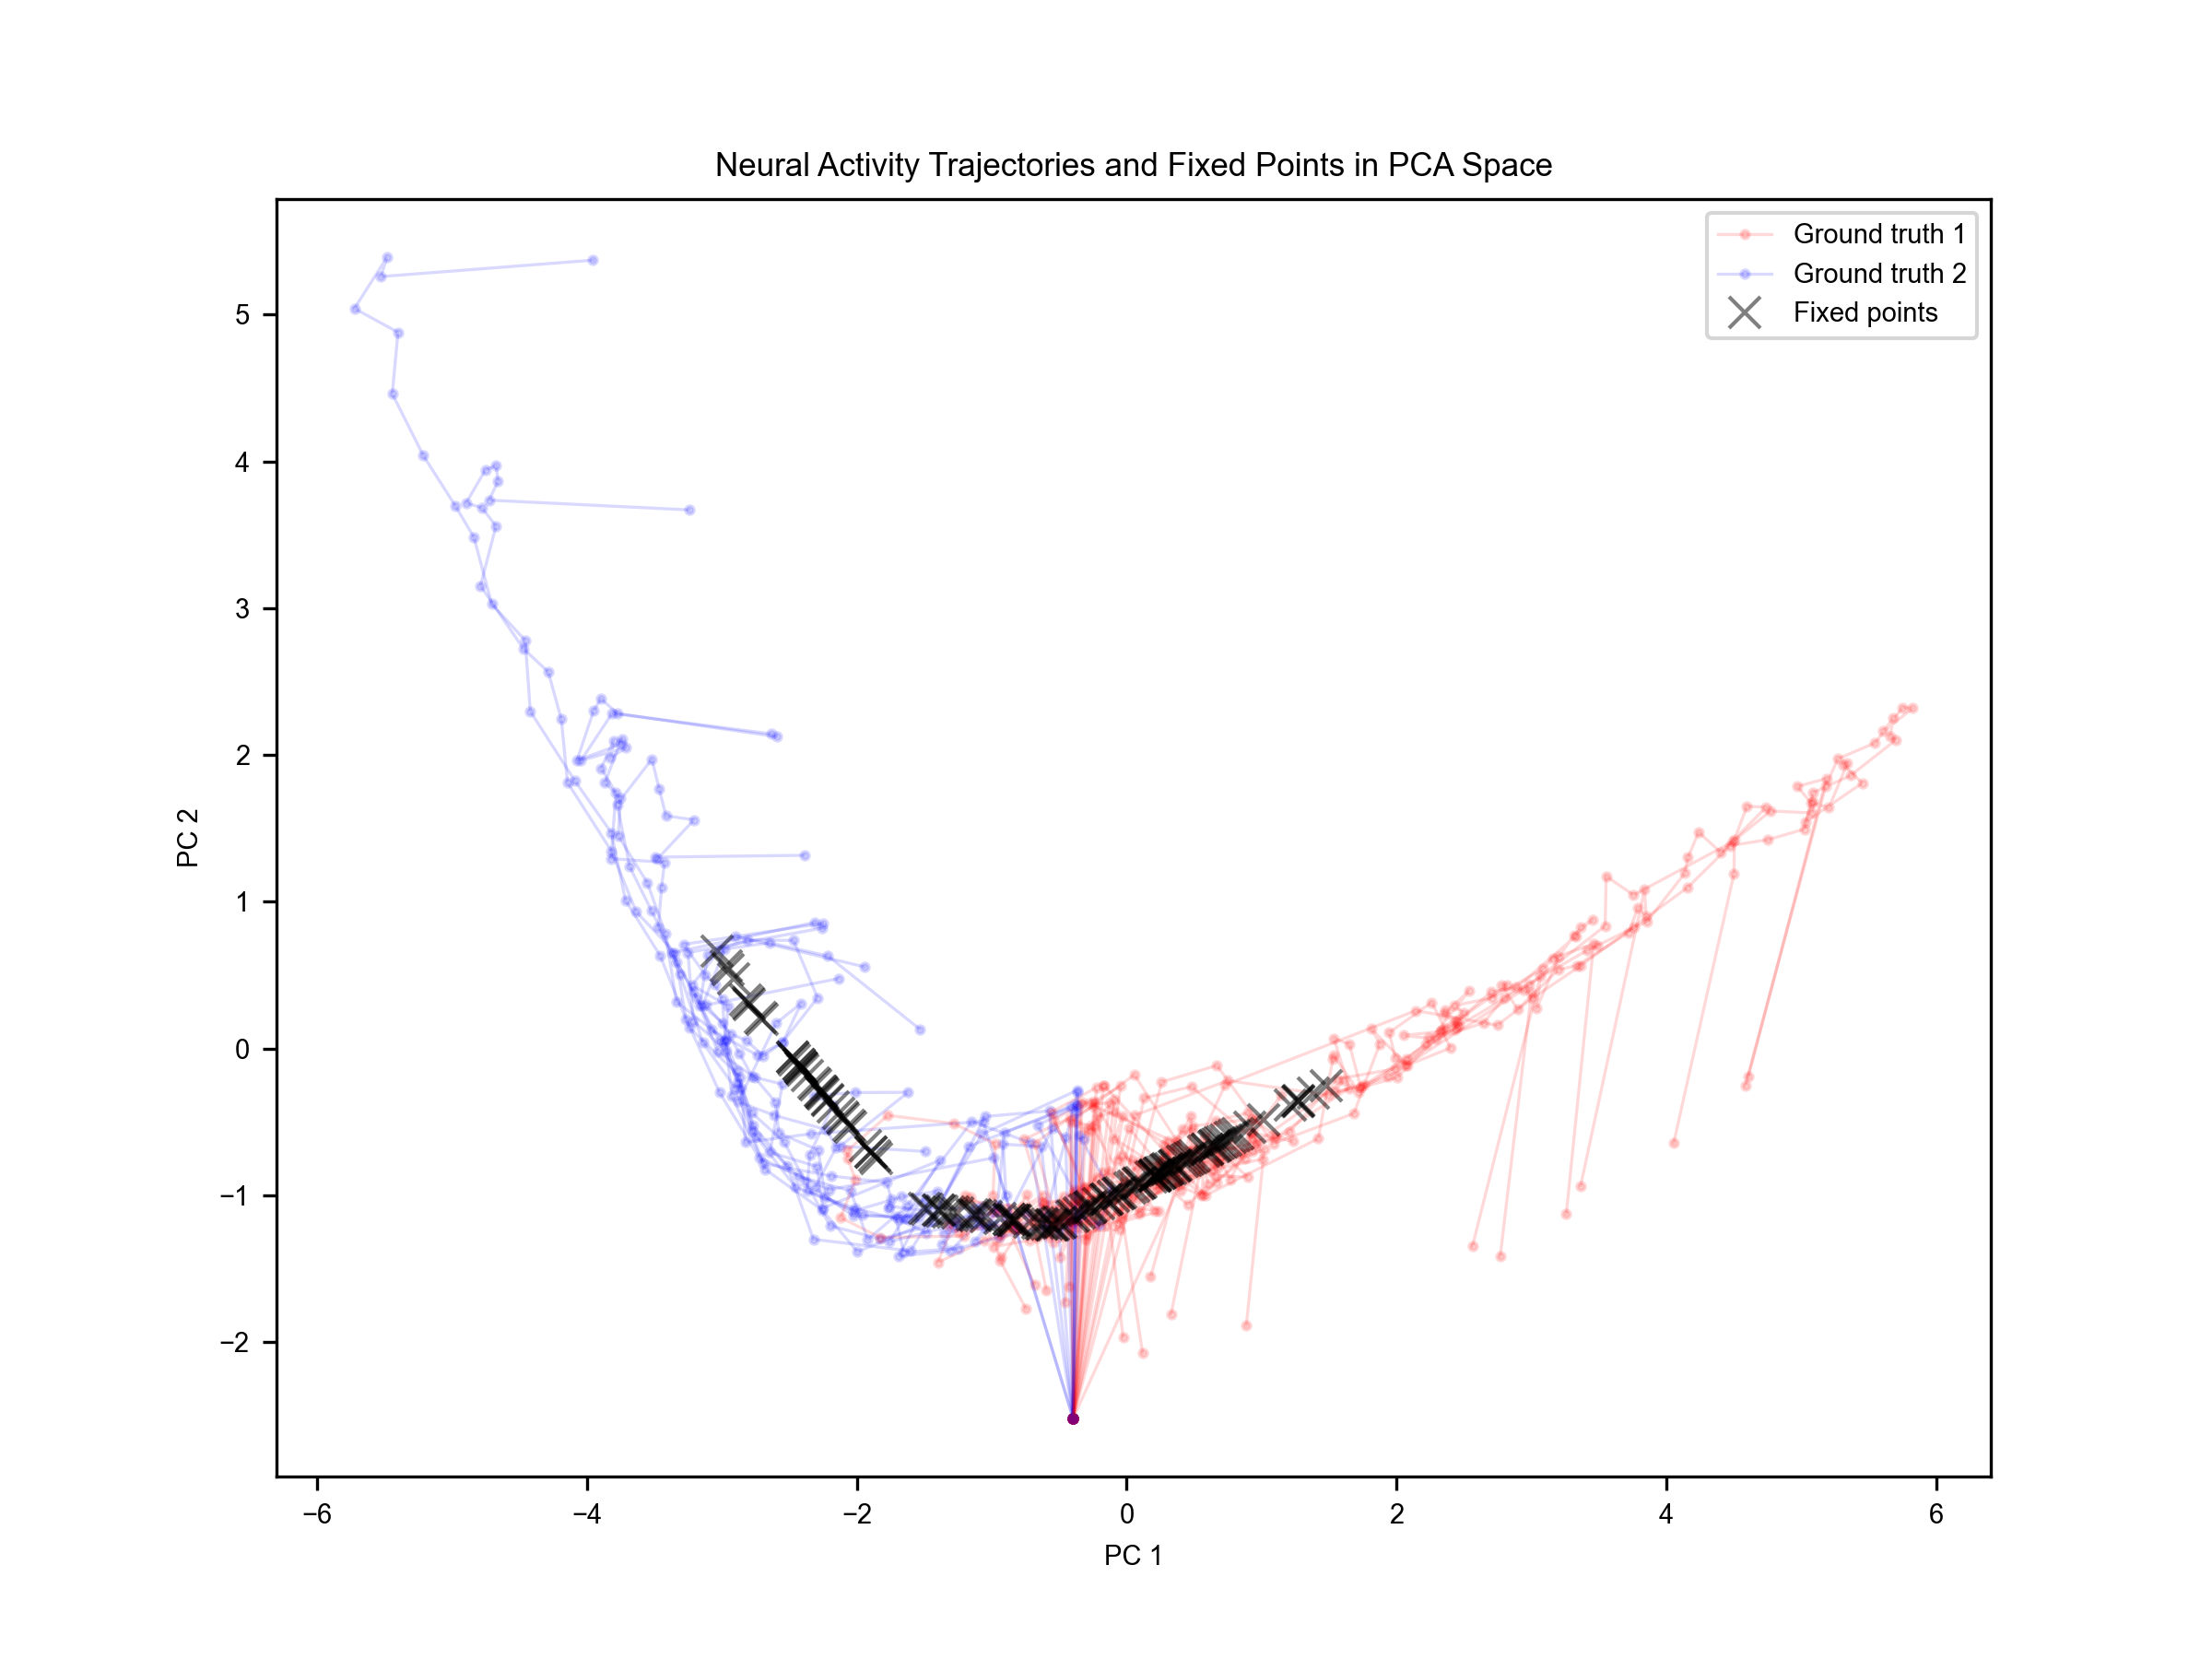
\includegraphics[width=0.8\textwidth]{pca_fixedpoints.png}
\caption{Fixed points analysis of the trained RNN. Black crosses (×) represent the 128 identified fixed points projected onto the first two principal components, forming a continuous 1D manifold. Trial trajectories for leftward (red) and rightward (blue) motion stimuli closely follow this manifold, indicating that the network implements evidence accumulation through a line attractor mechanism. The two ends of the manifold correspond to stable attractors representing the final categorical decisions, while intermediate points along the curve represent different levels of accumulated evidence. This architecture enables robust memory of accumulated evidence and categorical decision-making despite neural noise.}
\label{fig:fixed_point_manifold}
\end{figure}


\end{document}